

           %----------------%
\chapter{~~Internal details}\label{\numb section 12}
           %----------------%

This section contains material intended to assist the developer in reading the source code
of \maniFEM.
It contains mainly drawings which document specific parts of \maniFEM.


          %-------------------%
\section{~~\cinza{[empty]}}\label{\numb section 12.\numb parag 1}
          %-------------------%


          %----------------------------%
\section{~~Building a chain of segments}\label{\numb section 12.\numb parag 2}
          %----------------------------%

One of the simplest meshes is an open chain of segments.
The {\small\tt \verm{Mesh}} constructor with {\small\tt \textcolor{tag}{tag}::segment}
calls the {\small\tt\verm{Mesh}::build} method with {\small\tt \textcolor{tag}{tag}::segment}.
This method is defined in
{\small\tt global.cpp}, receives two vertices (a negative one and a positive one)
and the desired number of segments and builds the chain.
New vertices are built by using the constructor\hfil\break
{\small\tt \verm{Cell}} {\small\tt(} {\small\tt\textcolor{tag}{tag}::vertex} {\small\tt)}.
Space coordinates of each new vertex are defined by interpolating the coordinates of the
two extremities of the chain.
New segments are built by means of constructor {\small\tt \verm{Cell}} {\small\tt(}
{\small\tt\textcolor{tag}{tag}::segment,} {\small\tt A,} {\small\tt B} {\small\tt )},
where {\small\tt A} is a {\small\tt \verm{Cell}::Negative::Vertex} and {\small\tt B} is a
{\small\tt \verm{Cell}::Positive::Vertex}.

Note that the interpolation operation is a method belonging to {\small\tt working\_\,manifold}
(an object of the class {\small\tt Manifold}).
For a Euclidian manifold, this is just a convex combination of the values of the coordinates.
However, for other manifolds it may be a more complex operation.
For an implicit manifold, it involves a projection operation, as explained in paragraph
\ref{\numb section 8.\numb parag 1}.


          %---------------------------%
\section{~~Building a rectangular mesh}\label{\numb section 12.\numb parag 3}
          %---------------------------%

Constructor {\small\tt \verm{Mesh}::Mesh} {\small\tt(} {\small\tt\textcolor{tag}{tag}::rectangle,...)}
calls the {\small\tt\verm{Mesh}::build} method with {\small\tt \textcolor{tag}{tag}::rectangle}.
This method, defined in {\small\tt global.cpp}, builds a rectangular mesh from its
four sides (which are one-dimensional meshes, more precisely, open chains of segments).
No need to provide the number of divisions, the four sides already have their internal divisions.
Of course, opposite sides should have the same number of (segment) cells.

Paragraphs \ref{\numb section 1.\numb parag 4}, \ref{\numb section 1.\numb parag 5} and
many others (e.g. in section \ref{\numb section 2}) show the use of this constructor.

Actually, the name {\small\tt rectangle} is misleading.
Perhaps a better name would be {\small\tt quadrangle} but even this is not general enough to
describe the constructor's ability to build curved patches like the ones shown in paragraphs
\ref{\numb section 1.\numb parag 1} or \ref{\numb section 2.\numb parag 7} --
\ref{\numb section 2.\numb parag 11}.
Tags {\small\tt rectangle}, {\small\tt quadrangle} and {\small\tt quadrilateral} can be used
interchangeably.

\begin{figure}[ht] \centering
  \psfrag{A}{\small\tt\textcolor{textindraw}{A}}
  \psfrag{B}{\small\tt\textcolor{textindraw}{B}}
  \psfrag{C}{\small\tt\textcolor{textindraw}{C}}
  \psfrag{D}{\small\tt\textcolor{textindraw}{D}}
  \psfrag{south}{\small\tt\textcolor{textindraw}{south}}
  \psfrag{east}{\small\tt\textcolor{textindraw}{east}}
  \psfrag{north}{\small\tt\textcolor{textindraw}{north}}
  \psfrag{west}{\small\tt\textcolor{textindraw}{west}}
  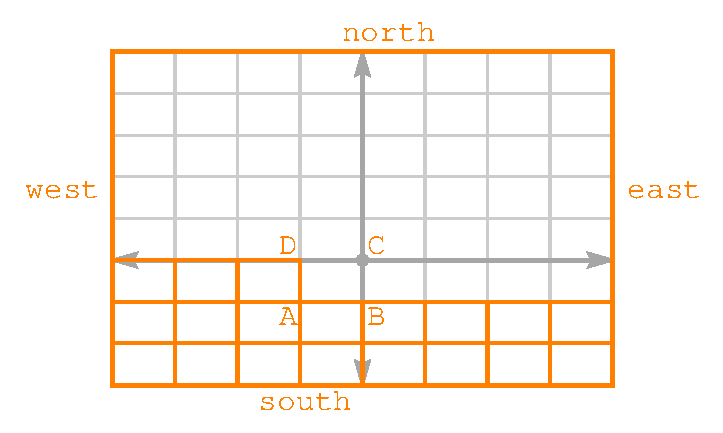
\includegraphics[width=90mm]{fig-rectangle}
  \caption{Meshing a rectangle}
  \label{\numb section 12.\numb fig 1}
\end{figure}

The coordinates of each new vertex are defined by interpolating the coordinates of four vertices
on the four given sides, as shown in figure \ref{\numb section 12.\numb fig 1}.
The complicated formula for the coefficients (involving $ \alpha^3 $ and $ \beta^3 $) is there
to ensure a smooth transition for the distribution of inner vertices in the case of non-uniform
distribution along one or several sides.
Paragraphs \ref{\numb section 2.\numb parag 1}, \ref{\numb section 2.\numb parag 9} and
\ref{\numb section 2.\numb parag 11} show examples where this is useful.

The remarks made in paragraph \ref{\numb section 12.\numb parag 2} about
the interpolation operation hold here.
Paragraph \ref{\numb section 2.\numb parag 7} shows an example where the interpolation operation
consists of a convex combination followed by a projection.
For a manifold defined through an external parameter, the convex combination is performed
on the external parameter and then the space coordinates are computed accordingly
(paragraph \ref{\numb section 2.\numb parag 18} shows such a situation).

Providing a {\small\tt \textcolor{tag}{tag}::with\_\,triangles} makes the constructor cut each rectangle
in halves; results are shown in paragraphs \ref{\numb section 2.\numb parag 3} and
\ref{\numb section 2.\numb parag 8}.


          %--------------------------%
\section{~~Building a triangular mesh}\label{\numb section 12.\numb parag 4}
          %--------------------------%

Building a triangular mesh involves an algorithm much alike the one for a rectangular mesh.
A noteworthy difference is that the interpolation operation involves now six vertices on
the boundary of the triangle, as shown in figure below.

\begin{figure}[ht] \centering
  \psfrag{A}{\small\tt\textcolor{textindraw}{A}}
  \psfrag{B}{\small\tt\textcolor{textindraw}{B}}
  \psfrag{C}{\small\tt\textcolor{textindraw}{C}}
  \psfrag{S}{\small\tt\textcolor{textindraw}{S}}
  \psfrag{P_AB}{\small\tt\textcolor{textindraw}{P\_\,AB}}
  \psfrag{Q_AB}{\small\tt\textcolor{textindraw}{Q\_\,AB}}
  \psfrag{P_BC}{\small\tt\textcolor{textindraw}{P\_\,BC}}
  \psfrag{Q_BC}{\small\tt\textcolor{textindraw}{Q\_\,BC}}
  \psfrag{P_CA}{\small\tt\textcolor{textindraw}{P\_\,CA}}
  \psfrag{Q_CA}{\small\tt\textcolor{textindraw}{Q\_\,CA}}
  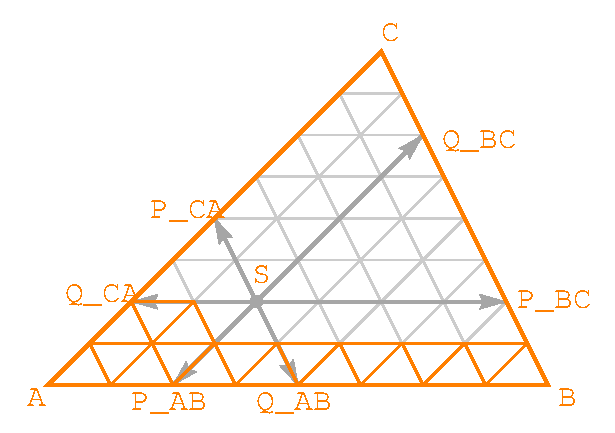
\includegraphics[width=75mm]{fig-triangle}
  \caption{Meshing a triangle}
  \label{\numb section 12.\numb fig 2}
\end{figure}

The coefficients for the interpolation have simpler formulas when compared with the ones in the
constructor of a rectangle (presented in paragraph \ref{\numb section 12.\numb parag 3});
the fact that we interpolate from six vertices compensates that.

Examples are presented in paragraphs \ref{\numb section 1.\numb parag 5},
\ref{\numb section 1.\numb parag 6} and \ref{\numb section 2.\numb parag 6}.


          %---------------------------%
\section{~~Progressive mesh generation}\label{\numb section 12.\numb parag 5}
          %---------------------------%

Several constructors {\small\tt \verm{Mesh}::Mesh} {\small\tt(}
{\small\tt\textcolor{tag}{tag}::progressive,...)} are defined in {\small\tt progressive.cpp};
they build a mesh on a given manifold starting with almost nothing.
More precisely, they start with the boundary of the future mesh, then they
move this interface with small steps, building the mesh behind it like a spider.
Actually, if the manifold is compact (like the sphere or the torus) and we want to mesh
all of it, there will be no boundary.
In this case we can start the process by providing nothing more than the manifold itself.
Section \ref{\numb section 3} gives several examples.

This is a complex process, much more complex than building a regular mesh of rectangles
(as described in paragraph \ref{\numb section 12.\numb parag 3}) or of triangles (as described
in paragraph \ref{\numb section 12.\numb parag 4}).
The constructor delegates the job to the function {\small\tt progressive\_\,construct}.

The mesh must follow the shape of the manifold; this is achieved by {\small\tt project}ing
newly created vertices on the working manifold, as explained in paragraph
\ref{\numb section 8.\numb parag 1}.

The initial interface may be disconnected.
Even if the initial interface is connected, it may become disconnected during the meshing
process, if it touches itself (paragraph \ref{\numb section 12.\numb parag 8}
discusses this event).

Detecting such touching points requires evaluating the distance between many pairs of points.
This may become extremely time consuming, unless special care is taken to organize points
belonging to the interface in a hierarchy allowing one to eliminate many pairs of points
from the evaluation process.
Paragraph \ref{\numb section 12.\numb parag 10} describes this hierarchy.

The next few paragraphs describe specific parts of this process of progressive mesh generation.


          %-----------%
\section{~~The normals}\label{\numb section 12.\numb parag 6}
          %-----------%

The meshing process described in paragraph \ref{\numb section 12.\numb parag 5} uses a set of
normal vectors.
Each segment in the interface has associated to it
a vector tangent to the working manifold and normal to the interface (we can
think of the interface as a curve embedded in that two-dimensional manifold).
These normal vectors provide the sense in which we want the mesh to grow (to the left or to
the right of the interface), that is, they define the orientation of the manifold and of
the mesh under construction.
They are used when we create a new vertex in order to decide its placement.

Actually, at the beginning of the process only one segment has an associated normal vector.
{\ManiFEM} then propagates this normal vector to the neighbour segments, walking along
the current connected component of the interface.
This means that, if there are other connected components, they will have no normal vectors.
When the current connected component of the interface touches other connected components
(this event is discussed in paragraph \ref{\numb section 12.\numb parag 8}), {\maniFEM}
% aproveita a oportunidade para ...
propagates the normal vectors to the new connected component.

Each time a new segment is added to the interface (this happens in situations described in
paragraphs \ref{\numb section 12.\numb parag 7} and \ref{\numb section 12.\numb parag 8}),
the normal associated to the new segment must be computed (propagated from neighbour
segments).


          %-----------------%
\section{~~Filling triangles}\label{\numb section 12.\numb parag 7}
          %-----------------%

Perhaps the simplest part of the meshing process described in paragraph
\ref{\numb section 12.\numb parag 5} is just walking along the interface and
adding new triangles.

A trivial case is when an angle is encountered which is close to $ 60^\circ $
(see figure below left).
Then we only have to fill the space with a new triangle.
Of course, before creating this new triangle a new segment {\small\tt AB} must be created
(no new vertex is needed).
Two old segments must be removed from the interface and the new one must be added.
Its normal must be computed (see paragraph \ref{\numb section 12.\numb parag 6}).

\begin{figure}[ht] \centering
  \psfrag{A}{\small\tt\textcolor{textindraw}{A}}
  \psfrag{B}{\small\tt\textcolor{textindraw}{B}}
  \psfrag{P}{\small\tt\textcolor{textindraw}{P}}
  \psfrag{point60}{\small\tt\textcolor{textindraw}{point\_\,60}}
  \psfrag{point120}{\small\tt\textcolor{textindraw}{point\_\,120}}
\begin{subfigure}{71mm}\centering
  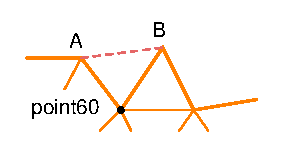
\includegraphics[width=55mm]{fill-angle-60}
\end{subfigure}  
\begin{subfigure}{71mm}\centering
  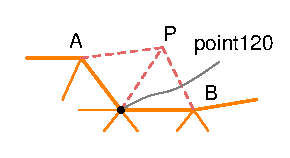
\includegraphics[width=55mm]{fill-angle-120}
\end{subfigure}  
  \caption{Filling a $ 60^\circ $ angle and a $ 120^\circ $ angle}
  \label{\numb section 12.\numb fig 3}
\end{figure}

A more complicated situation is when an angle is encountered which is close to $ 120^\circ $
(see figure above right).
A new vertex {\small\tt P} is created; its position is defined based on the two normals
of the adjacent segments.
Two new segments {\small\tt AP} and {\small\tt BP} are created,
then two new triangles are created and added to the mesh under construction.
Two old segments are removed from the interface then {\small\tt AP} and {\small\tt BP} are added
to the interface (their normals must be computed).

Special situations must be dealt with.
For instance, if one or both neighbour angles are also close to $ 120^\circ $,
we must take more vertices into account when we place the newly created vertex {\small\tt P};
figure \ref{\numb section 12.\numb fig 4} shows such situations.

\begin{figure}[ht] \centering
\begin{subfigure}{60mm}\centering
  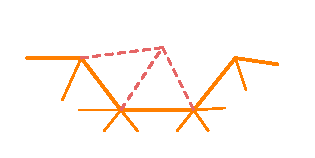
\includegraphics[width=55mm]{fill-angle-120-a}
\end{subfigure}  
\begin{subfigure}{50mm}\centering
  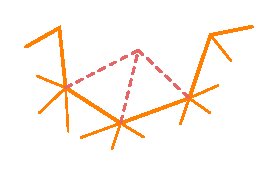
\includegraphics[width=45mm]{fill-angle-120-b}
\end{subfigure}  
  \caption{Two adjacent $ 120^\circ $ angles}
  \label{\numb section 12.\numb fig 4}
\end{figure}

Finally, if all angles of the current connected component of the interface are wide,
we may want to create a triangle ``out of the blue'', like in figure
\ref{\numb section 12.\numb fig 5}.

\begin{figure}[ht] \centering
  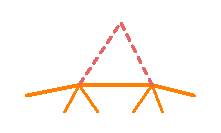
\includegraphics[width=45mm]{fill-blue}
  \caption{Creating a new triangle}
  \label{\numb section 12.\numb fig 5}
\end{figure}

Every time a new vertex is created, we must check whether it came close to another
zone of the interface and take action as described in paragraph
\ref{\numb section 12.\numb parag 8}.


          %----------------------%
\section{~~Touching the interface}\label{\numb section 12.\numb parag 8}
          %----------------------%

During the meshing process described in paragraph \ref{\numb section 12.\numb parag 5},
distinct zones of the moving interface may
come close to each other and the algorithm will eventually put them in contact.
Figure below shows the situation just prior to the contact.
The two zones may belong to different connected components of the interface,
as in the configuration shown below on the left.
In this case, the two components will merge, producing a new chain.
The normal vectors will be propagated to the segments which did not have an associated
normal vector (see paragraph \ref{\numb section 12.\numb parag 6}).
But it may also happen that they are part of the same connected component,
see the drawing below on the right.
In this case, the current chain will split in two.

\begin{figure}[ht] \centering
\begin{subfigure}{65mm}\centering
  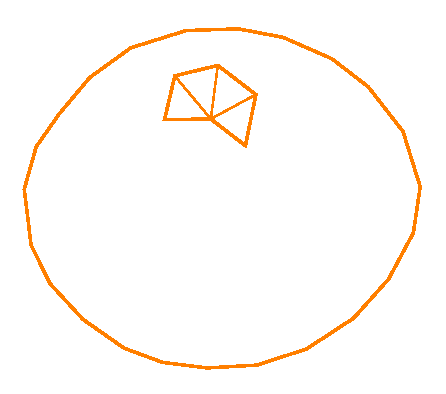
\includegraphics[width=52mm]{touching-interf-1}
\end{subfigure}  
\begin{subfigure}{65mm}\centering
  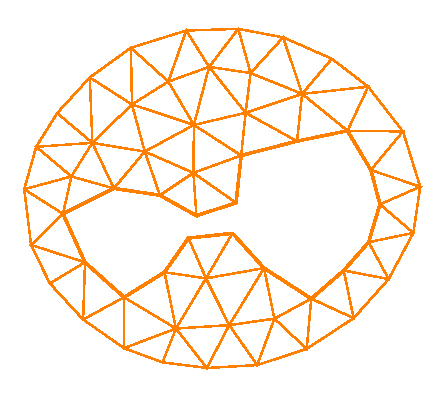
\includegraphics[width=52mm]{touching-interf-2}
\end{subfigure}  
  \caption{When the interface touches itself}
  \label{\numb section 12.\numb fig 6}
\end{figure}

Paragraphs \ref{\numb section 12.\numb parag 10} and \ref{\numb section 12.\numb parag 11}
explain how the {\small\tt\verm{MetricTree}} optimizes the process of checking whether a
certain vertex has come close to other vertices.

Methods {\small\tt glue\_\,two\_\,segs\_\,S} and
{\small\tt glue\_\,two\_\,segs\_\,Z} deal with two possible ways in which two
zones of the interface may touch,
independently of whether the two zones belong to the same connected component or not.
In the drawing below on the right hand side an S-shaped connection is created,
while in the other drawing a Z-shaped connection is created.

\begin{figure}[ht] \centering
  \psfrag{A}{\small\tt\textcolor{textindraw}{A}}
  \psfrag{B}{\small\tt\textcolor{textindraw}{B}}
  \psfrag{C}{\small\tt\textcolor{textindraw}{C}}
  \psfrag{D}{\small\tt\textcolor{textindraw}{D}}
\begin{subfigure}{45mm}\centering
  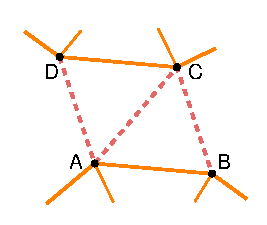
\includegraphics[width=40mm]{connect-S}
\end{subfigure}  
\begin{subfigure}{70mm}\centering
  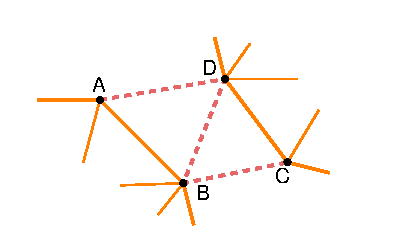
\includegraphics[width=65mm]{connect-Z}
\end{subfigure}  
  \caption{An S-shaped connection on the right, a Z-shaped connection on the left}
  \label{\numb section 12.\numb fig 7}
\end{figure}


          %------------------%
\section{~~\cinza{[empty]}}\label{\numb section 12.\numb parag 9}
          %------------------%


%---------%
\section{~~The cloud}\label{\numb section 12.\numb parag 10}
          %---------%

During the mesh generation process described in paragraph \ref{\numb section 12.\numb parag 5},
we have to check frequently the distance between
some vertex on the evolving interface and all other vertices of the interface
(including other connected components).
A direct comparison with all vertices would be very time consuming, so we rely on a tree-like
structure which we call {\small\tt\verm{MetricTree}} and which eliminates many vertices from the list
of candidates.%
\footnote {{\footnotesize\tt MetricTree} is also available separately at
{\footnotesize\tt https://github.com/cristian-barbarosie/MetricTree}}

The {\small\tt\verm{MetricTree}} is similar to quad- and oct-trees with two differences :
there is no assumption on the geometric dimension and the zones overlap.
It is similar to m-trees, just not balanced.

It works for a general metric space.
Triangular inequality is assumed, as well as symmetry.
Because it is not balanced, it deals well with non uniform clouds of points, that is,
with clouds having zones with
high density of points along with zones where the points are spread at large distances.

There is no upper limit on the number of children.
Actually, the average number of children can be used as a hint about the dimension of the
metric space (in the spirit of Hausdorff dimension).

{\small\tt \verm{MetricTree}} has been implemented with the intent of having wide usability,
independently of \maniFEM.
It is templated over the type of {\small\tt Point}s (the metric space) and over a callable
object returning the square of the distance between any two {\small\tt Point}s.
However, it still needs the touch of someone experienced in the subtleties of {\tt C++}.
Help is welcome.

We focus on the square of the distance rather than on the distance itself because it
is numerically cheaper (we prefer not to compute square roots).
Of course there are parts of the code where the true distance must be used
(e.g. when it comes to the triangular inequality).
Even there, simple algebraic manipulations allow us to avoid computing any square root.

The user interacts with the {\small\tt\verm{MetricTree}} through four methods.
The constructor sets the rank-zero distance and the ratio between successive
distances (see below).
Method {\small\tt add} adds a {\small\tt Point} to the cloud and returns a pointer to a
{\small\tt Node} which the user must keep and later provide to the {\small\tt remove} method.
The {\small\tt remove} method removes a {\small\tt Node} from the {\small\tt\verm{MetricTree}}.
Finally, and most importantly, method {\small\tt find\_\,close\_\,neighbours\_\,of} receives a
{\small\tt Point P} and a distance threshold and returns a list of {\small\tt Node}s near
{\small\tt P}.
It is irrelevant whether {\small\tt P} belongs or not to the cloud (if it belongs, it will
show up in the returned list, disguised as a {\small\tt Node}).
The user can recover (a copy of) the {\small\tt Point} from a {\small\tt Node} using the attribute
{\small\tt point}.
We have not implemented a method for finding the $n$ nodes closest to a given point
(we do not need such an operation for progressive mesh generation).

It is assumed that {\small\tt Point}s are cheap to copy.
If this is not the case for your {\small\tt Point}s, use pointers.
{\ManiFEM} uses wrappers, which are a sort of pointers (see paragraph
\ref{\numb section 11.\numb parag 4}).

Each node represents a point.
Leaves have no special status.
Each node has a rank which is an integer, possibly zero, possibly negative.
Children of a node {\small\tt N} have rank equal to {\small\tt rank[N] - \laranja{1}}.
Nodes with rank zero have no special status.
Leaves may have any rank, positive, zero or negative.
There is a {\small\tt root} of course (a node with no parent).
The root has the highest rank.
Even the rank of the root may be negative.

To each rank there is a distance {\small\tt dist} associated.
Children of a node {\small\tt N} are no farther than {\small\tt dist[rank[N]]} from {\small\tt N}.
Note that a point {\small\tt P} being at distance less than {\small\tt dist[rank[N]]} from
{\small\tt N} does not imply that {\small\tt P} must be a child (not even an indirect descendant)
of {\small\tt N}.
In other words : zones overlap.

{\small\tt dist[k]} is a geometric sequence with ratio {\small\tt ratio}.
{\small\tt ratio} must be greater than two; we recommend some value between 5 and 10.
So, {\small\tt dist[k] == ratio}$^{\hbox{\footnotesize\tt k }}${\small\tt dist[\laranja{0}]}.
Recall that {\small\tt k} may be negative.

Besides the {\small\tt dist}ance, to each rank {\small\tt k} we associate a {\small\tt range}
which represents the sum of distances of that rank and of all lower ranks.
That is,
\begin{Verbatim}[commandchars=\\\{\},formatcom=\small\tt,baselinestretch=0.94]
   range[k] == dist[k] / ( \laranja{1} - \laranja{1} / ratio )\,; \ range[k] > dist[k].
\end{Verbatim}
\noindent This means that an indirect descendant of a node {\small\tt N} cannot be farther than
{\small\tt range[rank[N]]} from {\small\tt N}.
Again, the reverse may be false.

\begin{figure}[ht] \centering
  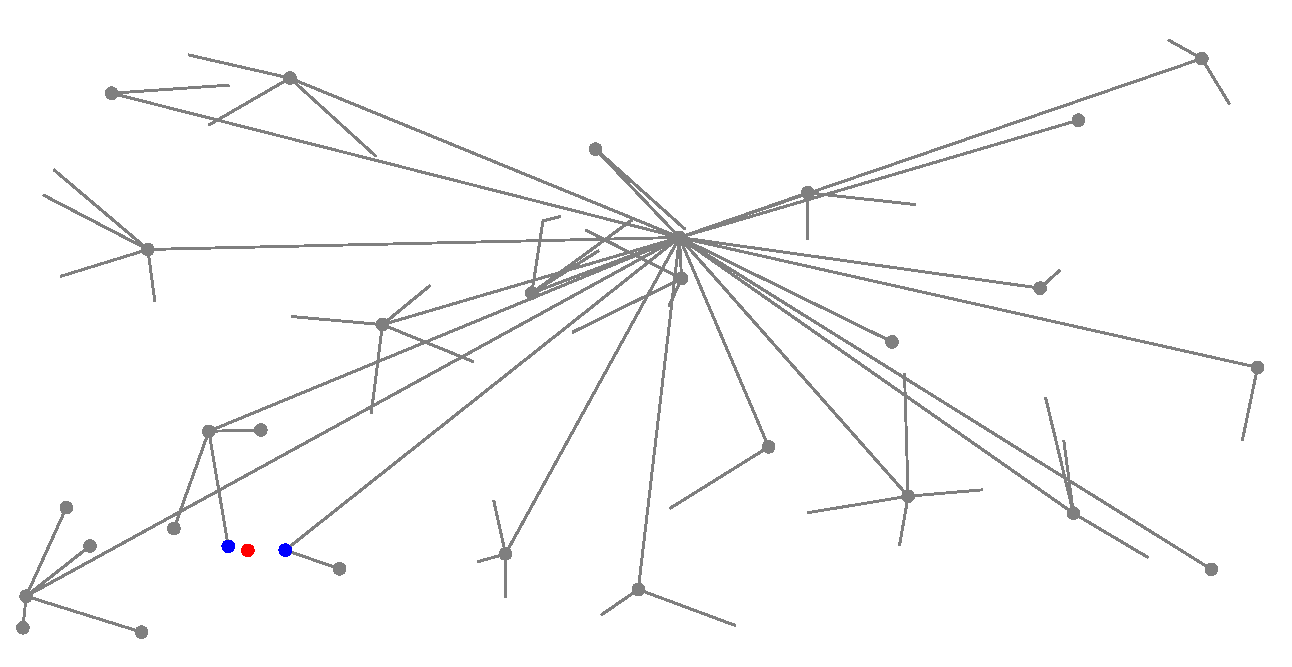
\includegraphics[width=110mm]{metric-tree}
  \caption{Metric tree}
  \label{\numb section 11.\numb fig 3}
\end{figure}

Figure \ref{\numb section 11.\numb fig 3} shows a cloud of (randomly generated) points in
$ \mathbb{R}^2 $ organized in a {\small\tt\verm{MetricTree}}.
It also illustrates the process of {\small\tt find\_\,close\_\,neighbours\_\,of} a given point.
This method takes two arguments : a {\small\tt Point} (drawn in red) and a distance.
It returns a list (drawn in blue) of all {\small\tt Node}s in the cloud which are close enough
to the red point (closer than the given distance).
It is irrelevant whether the red point belongs to the cloud or not;
if it belongs, it will be returned as element of the list.

Figure \ref{\numb section 11.\numb fig 3} shows grey dots at nodes which have been analysed
during the process of {\small\tt find\_\,close\_\,neighbours}
x(their distance to the red dot has been computed).
Lines without a dot represent nodes in the {\small\tt\verm{MetricTree}} which have not even been
looked at because their parent has decided (based on the triangular inequality)
that they cannot be close enough to the red dot.
Their distance to the red point has not been computed, thus alleviating the computational
burden.

If you want to run this example on your computer, it suffices to download three files
({\small\tt Makefile}, {\small\tt metric-tree-verbose.h} and
{\small\tt test-\ref{\numb section 12.\numb parag 10}.cpp}) from\hfil\break
{\small\tt https://github.com/cristian-barbarosie/manifem},\hfil\break
then {\small\tt make run-\ref{\numb section 12.\numb parag 10}}.


          %----------------------------------------%
\section{~~The cloud in progressive mesh generation}\label{\numb section 12.\numb parag 11}
          %----------------------------------------%

The use of {\small\tt\verm{MetricTree}} for progressive mesh generation (described in paragraph
\ref{\numb section 12.\numb parag 5}, with examples in section \ref{\numb section 3})
is tricky when we are meshing a submanifold of $ \mathbb{R}^n $
(a curve in $ \mathbb{R}^2 $ or $ \mathbb{R}^3 $, a surface in $ \mathbb{R}^3 $)
because there are two distances we must deal with.
There is the global, Euclidian, distance in the surrounding space
and there is the local distance on the tangent space of the manifold.
They are equal locally (at short distances) unless we attach a specific Riemann metric
to the manifold as shown in paragraphs \ref{\numb section 3.\numb parag 23} and
\ref{\numb section 3.\numb parag 24}.

Even if we don't play with a specific Riemann metric, the Euclidian metric is different,
at large distances, from the metric on the manifold defined by means of geodesics.
And anyway, computing the distance by means of geodesics is not affordable (it is too heavy
computationally).

We have chosen the following work-out.
We use a {\small\tt\verm{MetricTree}} with (the square of) the usual Euclidian distance
(which is computationally cheap).
This means that a call to {\small\tt\verm{MetricTree}:: ::find\_\,close\_\,neighbours\_\,of}
will produce a list which is too large in the sense that it may contain points which are
farther than the distance given as argument.
The calling program must then filter this list by measuring distances with the local metric.
The difference shouldn't be important if we are careful to choose the {\small\tt
desired\_\,distance} (be it a constant or a function) small when compared with the curvature
of the manifold (see paragraph \ref{\numb section 3.\numb parag 16}).

If we define a non-uniform Riemann metric
(as in paragraph \ref{\numb section 3.\numb parag 23}),
we must call {\small\tt find\_\,close\_\, \_\,neighbours\_\,of} with a modified value of the
distance.
If we define an anisotropic Riemann metric
(as in paragraph \ref{\numb section 3.\numb parag 24}),
we need a lower bound on the Rayleigh coefficient of the matrix $M$ (i.e.\ a lower bound
on its eigenvalues, or, equivalently, an upper bound of the spectral radius of the inverse
matrix) for computing the modified value to provide to {\small\tt find\_\,close\_\,neighbours\_\,of}.
Providing separately the {\small\tt principal\_\,part} and the {\small\tt deviatoric\_\,part} helps.
The {\small\tt principal\_\,part} is a positive scalar, while {\small\tt deviatoric\_\,part} is
a matrix responsible for the anisotropy; this matrix should be semi-definite positive.
Desirably, the {\small\tt deviatoric\_\,part} should be a singular matrix (having a null eigenvalue);
this way, the lower bound on the Rayleigh coefficient is simply the {\small\tt principal\_\,part}.
If we provide only the sum $M$, {\maniFEM} will compute, at each step, the lower bound on the
Rayleigh coefficient, which may be a heavy computational burden.
When the metric is highly anisotropic, the list returned by method
{\small\tt find\_\,close\_\,neighbours\_\,of} will be singnificantly larger than the correct,
filtered, list.

